\documentclass{standalone}
\usepackage{tikz}
\usetikzlibrary{patterns, positioning}


\begin{document}
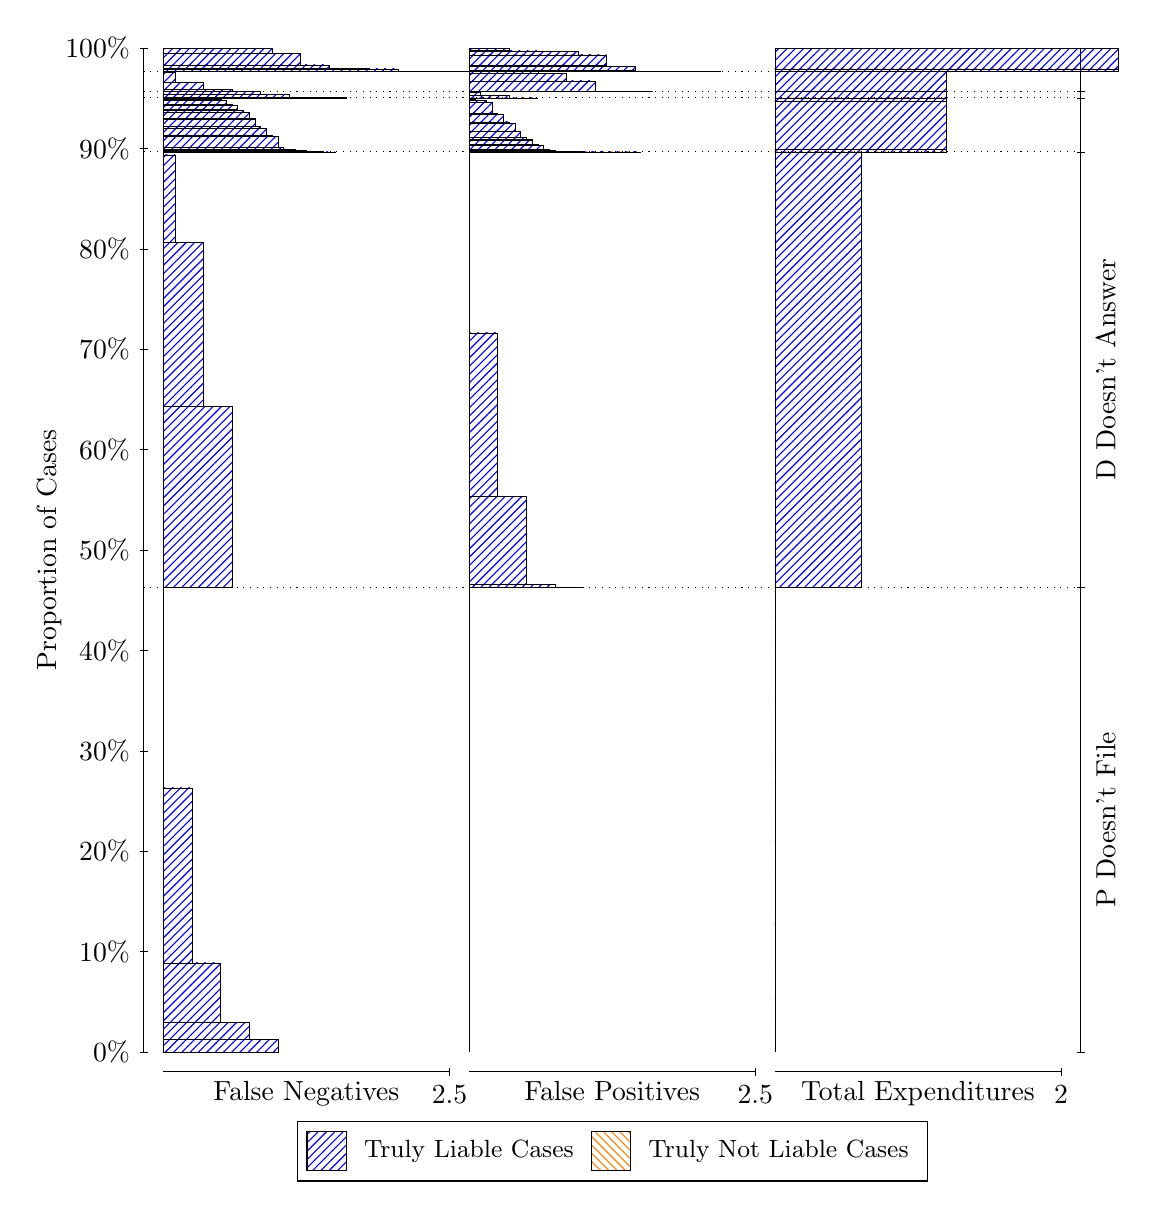
\begin{tikzpicture}
\draw[black, very thin] (1.5,1.75) -- (1.5,14.5);
\node[rotate=90, text=black, anchor=center] at (0.3, 8.125) {Proportion of Cases};
\draw[black, very thin] (1.45,1.75) -- (1.55,1.75);
\node[text=black, anchor=east] at (1.45, 1.75) {0\%};
\draw[black, very thin] (1.45,3.025) -- (1.55,3.025);
\node[text=black, anchor=east] at (1.45, 3.025) {10\%};
\draw[black, very thin] (1.45,4.3) -- (1.55,4.3);
\node[text=black, anchor=east] at (1.45, 4.3) {20\%};
\draw[black, very thin] (1.45,5.575) -- (1.55,5.575);
\node[text=black, anchor=east] at (1.45, 5.575) {30\%};
\draw[black, very thin] (1.45,6.85) -- (1.55,6.85);
\node[text=black, anchor=east] at (1.45, 6.85) {40\%};
\draw[black, very thin] (1.45,8.125) -- (1.55,8.125);
\node[text=black, anchor=east] at (1.45, 8.125) {50\%};
\draw[black, very thin] (1.45,9.4) -- (1.55,9.4);
\node[text=black, anchor=east] at (1.45, 9.4) {60\%};
\draw[black, very thin] (1.45,10.675) -- (1.55,10.675);
\node[text=black, anchor=east] at (1.45, 10.675) {70\%};
\draw[black, very thin] (1.45,11.95) -- (1.55,11.95);
\node[text=black, anchor=east] at (1.45, 11.95) {80\%};
\draw[black, very thin] (1.45,13.225) -- (1.55,13.225);
\node[text=black, anchor=east] at (1.45, 13.225) {90\%};
\draw[black, very thin] (1.45,14.5) -- (1.55,14.5);
\node[text=black, anchor=east] at (1.45, 14.5) {100\%};

\draw[black, very thin] (13.4,1.75) -- (13.4,14.5);
\draw[black, very thin] (13.35,1.75) -- (13.45,1.75);
\node[anchor=west] at (13.35, 1.75) {};
\draw[black, very thin] (13.35,7.651) -- (13.45,7.651);
\node[anchor=west] at (13.35, 7.651) {};
\draw[black, very thin] (13.35,13.181) -- (13.45,13.181);
\node[anchor=west] at (13.35, 13.181) {};
\draw[black, very thin] (13.35,13.868) -- (13.45,13.868);
\node[anchor=west] at (13.35, 13.868) {};
\draw[black, very thin] (13.35,13.945) -- (13.45,13.945);
\node[anchor=west] at (13.35, 13.945) {};
\draw[black, very thin] (13.35,14.199) -- (13.45,14.199);
\node[anchor=west] at (13.35, 14.199) {};
\draw[black, very thin] (13.35,14.5) -- (13.45,14.5);
\node[anchor=west] at (13.35, 14.5) {};

\draw[black, very thin, pattern color=blue, pattern=north east lines] (1.75,1.75) rectangle (3.2033,1.9086);
\draw[black, very thin, pattern color=blue, pattern=north east lines] (1.75,1.9086) rectangle (2.84,2.1216);
\draw[black, very thin, pattern color=blue, pattern=north east lines] (1.75,2.1216) rectangle (2.4767,2.8827);
\draw[black, very thin, pattern color=blue, pattern=north east lines] (1.75,2.8827) rectangle (2.1133,5.1043);
\draw[black, very thin, pattern color=orange, pattern=north west lines] (1.75,5.1043) rectangle (1.75,5.1043);
\draw[black, very thin, pattern color=blue, pattern=north east lines] (1.75,5.1043) rectangle (1.75,7.651);
\draw[black, very thin, pattern color=blue, pattern=north east lines] (1.75,7.651) rectangle (2.622,9.9507);
\draw[black, very thin, pattern color=blue, pattern=north east lines] (1.75,9.9507) rectangle (2.2587,12.027);
\draw[black, very thin, pattern color=blue, pattern=north east lines] (1.75,12.027) rectangle (1.8953,13.144);
\draw[black, very thin, pattern color=orange, pattern=north west lines] (1.75,13.144) rectangle (1.75,13.144);
\draw[black, very thin, pattern color=blue, pattern=north east lines] (1.75,13.144) rectangle (1.75,13.181);
\draw[black, very thin, pattern color=blue, pattern=north east lines] (1.75,13.181) rectangle (3.93,13.182);
\draw[black, very thin, pattern color=blue, pattern=north east lines] (1.75,13.182) rectangle (3.7847,13.183);
\draw[black, very thin, pattern color=blue, pattern=north east lines] (1.75,13.183) rectangle (3.6393,13.185);
\draw[black, very thin, pattern color=blue, pattern=north east lines] (1.75,13.185) rectangle (3.5667,13.198);
\draw[black, very thin, pattern color=blue, pattern=north east lines] (1.75,13.198) rectangle (3.494,13.2);
\draw[black, very thin, pattern color=blue, pattern=north east lines] (1.75,13.2) rectangle (3.4213,13.211);
\draw[black, very thin, pattern color=blue, pattern=north east lines] (1.75,13.211) rectangle (3.3487,13.215);
\draw[black, very thin, pattern color=blue, pattern=north east lines] (1.75,13.215) rectangle (3.276,13.238);
\draw[black, very thin, pattern color=blue, pattern=north east lines] (1.75,13.238) rectangle (3.2033,13.374);
\draw[black, very thin, pattern color=blue, pattern=north east lines] (1.75,13.374) rectangle (3.1307,13.388);
\draw[black, very thin, pattern color=blue, pattern=north east lines] (1.75,13.388) rectangle (3.058,13.396);
\draw[black, very thin, pattern color=blue, pattern=north east lines] (1.75,13.396) rectangle (3.058,13.487);
\draw[black, very thin, pattern color=blue, pattern=north east lines] (1.75,13.487) rectangle (2.9853,13.503);
\draw[black, very thin, pattern color=blue, pattern=north east lines] (1.75,13.503) rectangle (2.9127,13.597);
\draw[black, very thin, pattern color=blue, pattern=north east lines] (1.75,13.597) rectangle (2.9127,13.602);
\draw[black, very thin, pattern color=blue, pattern=north east lines] (1.75,13.602) rectangle (2.84,13.685);
\draw[black, very thin, pattern color=blue, pattern=north east lines] (1.75,13.685) rectangle (2.7673,13.707);
\draw[black, very thin, pattern color=blue, pattern=north east lines] (1.75,13.707) rectangle (2.6947,13.719);
\draw[black, very thin, pattern color=blue, pattern=north east lines] (1.75,13.719) rectangle (2.6947,13.771);
\draw[black, very thin, pattern color=blue, pattern=north east lines] (1.75,13.771) rectangle (2.622,13.787);
\draw[black, very thin, pattern color=blue, pattern=north east lines] (1.75,13.787) rectangle (2.5493,13.831);
\draw[black, very thin, pattern color=blue, pattern=north east lines] (1.75,13.831) rectangle (2.5493,13.841);
\draw[black, very thin, pattern color=blue, pattern=north east lines] (1.75,13.841) rectangle (2.4767,13.85);
\draw[black, very thin, pattern color=blue, pattern=north east lines] (1.75,13.85) rectangle (2.404,13.85);
\draw[black, very thin, pattern color=blue, pattern=north east lines] (1.75,13.85) rectangle (2.404,13.857);
\draw[black, very thin, pattern color=blue, pattern=north east lines] (1.75,13.857) rectangle (2.3313,13.861);
\draw[black, very thin, pattern color=blue, pattern=north east lines] (1.75,13.861) rectangle (2.3313,13.862);
\draw[black, very thin, pattern color=blue, pattern=north east lines] (1.75,13.862) rectangle (2.2587,13.862);
\draw[black, very thin, pattern color=blue, pattern=north east lines] (1.75,13.862) rectangle (2.186,13.863);
\draw[black, very thin, pattern color=blue, pattern=north east lines] (1.75,13.863) rectangle (2.186,13.865);
\draw[black, very thin, pattern color=blue, pattern=north east lines] (1.75,13.865) rectangle (2.1133,13.866);
\draw[black, very thin, pattern color=blue, pattern=north east lines] (1.75,13.866) rectangle (2.0407,13.866);
\draw[black, very thin, pattern color=blue, pattern=north east lines] (1.75,13.866) rectangle (2.0407,13.867);
\draw[black, very thin, pattern color=blue, pattern=north east lines] (1.75,13.867) rectangle (1.968,13.867);
\draw[black, very thin, pattern color=blue, pattern=north east lines] (1.75,13.867) rectangle (1.8953,13.867);
\draw[black, very thin, pattern color=blue, pattern=north east lines] (1.75,13.867) rectangle (1.8227,13.867);
\draw[black, very thin, pattern color=orange, pattern=north west lines] (1.75,13.867) rectangle (1.75,13.867);
\draw[black, very thin, pattern color=blue, pattern=north east lines] (1.75,13.867) rectangle (1.75,13.868);
\draw[black, very thin, pattern color=blue, pattern=north east lines] (1.75,13.868) rectangle (4.0753,13.869);
\draw[black, very thin, pattern color=blue, pattern=north east lines] (1.75,13.869) rectangle (3.712,13.874);
\draw[black, very thin, pattern color=blue, pattern=north east lines] (1.75,13.874) rectangle (3.3487,13.916);
\draw[black, very thin, pattern color=blue, pattern=north east lines] (1.75,13.916) rectangle (2.9853,13.945);
\draw[black, very thin, pattern color=blue, pattern=north east lines] (1.75,13.945) rectangle (2.622,13.945);
\draw[black, very thin, pattern color=orange, pattern=north west lines] (1.75,13.945) rectangle (1.75,13.945);
\draw[black, very thin, pattern color=blue, pattern=north east lines] (1.75,13.945) rectangle (2.622,13.97);
\draw[black, very thin, pattern color=blue, pattern=north east lines] (1.75,13.97) rectangle (2.2587,14.061);
\draw[black, very thin, pattern color=blue, pattern=north east lines] (1.75,14.061) rectangle (1.8953,14.194);
\draw[black, very thin, pattern color=orange, pattern=north west lines] (1.75,14.194) rectangle (1.75,14.194);
\draw[black, very thin, pattern color=blue, pattern=north east lines] (1.75,14.194) rectangle (1.75,14.199);
\draw[black, very thin, pattern color=blue, pattern=north east lines] (1.75,14.199) rectangle (5.8193,14.199);
\draw[black, very thin, pattern color=blue, pattern=north east lines] (1.75,14.199) rectangle (5.456,14.199);
\draw[black, very thin, pattern color=blue, pattern=north east lines] (1.75,14.199) rectangle (5.0927,14.203);
\draw[black, very thin, pattern color=blue, pattern=north east lines] (1.75,14.203) rectangle (4.7293,14.235);
\draw[black, very thin, pattern color=blue, pattern=north east lines] (1.75,14.235) rectangle (4.584,14.235);
\draw[black, very thin, pattern color=blue, pattern=north east lines] (1.75,14.235) rectangle (4.366,14.244);
\draw[black, very thin, pattern color=blue, pattern=north east lines] (1.75,14.244) rectangle (4.2207,14.244);
\draw[black, very thin, pattern color=blue, pattern=north east lines] (1.75,14.244) rectangle (4.0027,14.245);
\draw[black, very thin, pattern color=blue, pattern=north east lines] (1.75,14.245) rectangle (3.8573,14.285);
\draw[black, very thin, pattern color=blue, pattern=north east lines] (1.75,14.285) rectangle (3.6393,14.285);
\draw[black, very thin, pattern color=blue, pattern=north east lines] (1.75,14.285) rectangle (3.494,14.432);
\draw[black, very thin, pattern color=blue, pattern=north east lines] (1.75,14.432) rectangle (3.1307,14.495);
\draw[black, very thin, pattern color=blue, pattern=north east lines] (1.75,14.495) rectangle (2.7673,14.5);
\draw[black, very thin, pattern color=blue, pattern=north east lines] (1.75,14.5) rectangle (2.404,14.5);
\draw[black, very thin, pattern color=blue, pattern=north east lines] (1.75,14.5) rectangle (2.0407,14.5);
\draw[black, very thin, pattern color=orange, pattern=north west lines] (1.75,14.5) rectangle (1.75,14.5);
\draw[black, very thin, pattern color=orange, pattern=north west lines] (5.6333,1.75) rectangle (5.6333,1.75);
\draw[black, very thin, pattern color=blue, pattern=north east lines] (5.6333,1.75) rectangle (5.6333,7.651);
\draw[black, very thin, pattern color=orange, pattern=north west lines] (5.6333,7.651) rectangle (7.0867,7.651);
\draw[black, very thin, pattern color=blue, pattern=north east lines] (5.6333,7.651) rectangle (7.0867,7.651);
\draw[black, very thin, pattern color=blue, pattern=north east lines] (5.6333,7.651) rectangle (6.7233,7.6878);
\draw[black, very thin, pattern color=blue, pattern=north east lines] (5.6333,7.6878) rectangle (6.36,8.8053);
\draw[black, very thin, pattern color=blue, pattern=north east lines] (5.6333,8.8053) rectangle (5.9967,10.881);
\draw[black, very thin, pattern color=blue, pattern=north east lines] (5.6333,10.881) rectangle (5.6333,13.181);
\draw[black, very thin, pattern color=orange, pattern=north west lines] (5.6333,13.181) rectangle (7.8133,13.181);
\draw[black, very thin, pattern color=blue, pattern=north east lines] (5.6333,13.181) rectangle (7.8133,13.181);
\draw[black, very thin, pattern color=orange, pattern=north west lines] (5.6333,13.181) rectangle (7.668,13.181);
\draw[black, very thin, pattern color=blue, pattern=north east lines] (5.6333,13.181) rectangle (7.668,13.181);
\draw[black, very thin, pattern color=orange, pattern=north west lines] (5.6333,13.181) rectangle (7.5227,13.181);
\draw[black, very thin, pattern color=blue, pattern=north east lines] (5.6333,13.181) rectangle (7.5227,13.181);
\draw[black, very thin, pattern color=blue, pattern=north east lines] (5.6333,13.181) rectangle (7.45,13.181);
\draw[black, very thin, pattern color=orange, pattern=north west lines] (5.6333,13.181) rectangle (7.3773,13.181);
\draw[black, very thin, pattern color=blue, pattern=north east lines] (5.6333,13.181) rectangle (7.3773,13.181);
\draw[black, very thin, pattern color=blue, pattern=north east lines] (5.6333,13.181) rectangle (7.3047,13.181);
\draw[black, very thin, pattern color=orange, pattern=north west lines] (5.6333,13.181) rectangle (7.232,13.181);
\draw[black, very thin, pattern color=blue, pattern=north east lines] (5.6333,13.181) rectangle (7.232,13.181);
\draw[black, very thin, pattern color=blue, pattern=north east lines] (5.6333,13.181) rectangle (7.1593,13.181);
\draw[black, very thin, pattern color=orange, pattern=north west lines] (5.6333,13.181) rectangle (7.0867,13.181);
\draw[black, very thin, pattern color=blue, pattern=north east lines] (5.6333,13.181) rectangle (7.0867,13.183);
\draw[black, very thin, pattern color=blue, pattern=north east lines] (5.6333,13.183) rectangle (7.014,13.183);
\draw[black, very thin, pattern color=orange, pattern=north west lines] (5.6333,13.183) rectangle (6.9413,13.183);
\draw[black, very thin, pattern color=blue, pattern=north east lines] (5.6333,13.183) rectangle (6.9413,13.186);
\draw[black, very thin, pattern color=blue, pattern=north east lines] (5.6333,13.186) rectangle (6.8687,13.187);
\draw[black, very thin, pattern color=orange, pattern=north west lines] (5.6333,13.187) rectangle (6.796,13.187);
\draw[black, very thin, pattern color=blue, pattern=north east lines] (5.6333,13.187) rectangle (6.796,13.187);
\draw[black, very thin, pattern color=blue, pattern=north east lines] (5.6333,13.187) rectangle (6.796,13.191);
\draw[black, very thin, pattern color=blue, pattern=north east lines] (5.6333,13.191) rectangle (6.7233,13.199);
\draw[black, very thin, pattern color=orange, pattern=north west lines] (5.6333,13.199) rectangle (6.6507,13.199);
\draw[black, very thin, pattern color=blue, pattern=north east lines] (5.6333,13.199) rectangle (6.6507,13.208);
\draw[black, very thin, pattern color=blue, pattern=north east lines] (5.6333,13.208) rectangle (6.578,13.262);
\draw[black, very thin, pattern color=blue, pattern=north east lines] (5.6333,13.262) rectangle (6.5053,13.278);
\draw[black, very thin, pattern color=blue, pattern=north east lines] (5.6333,13.278) rectangle (6.4327,13.329);
\draw[black, very thin, pattern color=blue, pattern=north east lines] (5.6333,13.329) rectangle (6.4327,13.342);
\draw[black, very thin, pattern color=blue, pattern=north east lines] (5.6333,13.342) rectangle (6.36,13.363);
\draw[black, very thin, pattern color=blue, pattern=north east lines] (5.6333,13.363) rectangle (6.2873,13.446);
\draw[black, very thin, pattern color=blue, pattern=north east lines] (5.6333,13.446) rectangle (6.2147,13.546);
\draw[black, very thin, pattern color=blue, pattern=north east lines] (5.6333,13.546) rectangle (6.142,13.562);
\draw[black, very thin, pattern color=blue, pattern=north east lines] (5.6333,13.562) rectangle (6.0693,13.653);
\draw[black, very thin, pattern color=blue, pattern=north east lines] (5.6333,13.653) rectangle (6.0693,13.661);
\draw[black, very thin, pattern color=blue, pattern=north east lines] (5.6333,13.661) rectangle (5.9967,13.675);
\draw[black, very thin, pattern color=blue, pattern=north east lines] (5.6333,13.675) rectangle (5.924,13.811);
\draw[black, very thin, pattern color=blue, pattern=north east lines] (5.6333,13.811) rectangle (5.8513,13.833);
\draw[black, very thin, pattern color=blue, pattern=north east lines] (5.6333,13.833) rectangle (5.7787,13.838);
\draw[black, very thin, pattern color=blue, pattern=north east lines] (5.6333,13.838) rectangle (5.706,13.849);
\draw[black, very thin, pattern color=blue, pattern=north east lines] (5.6333,13.849) rectangle (5.6333,13.868);
\draw[black, very thin, pattern color=orange, pattern=north west lines] (5.6333,13.868) rectangle (6.5053,13.868);
\draw[black, very thin, pattern color=blue, pattern=north east lines] (5.6333,13.868) rectangle (6.5053,13.868);
\draw[black, very thin, pattern color=blue, pattern=north east lines] (5.6333,13.868) rectangle (6.142,13.896);
\draw[black, very thin, pattern color=blue, pattern=north east lines] (5.6333,13.896) rectangle (5.7787,13.938);
\draw[black, very thin, pattern color=blue, pattern=north east lines] (5.6333,13.938) rectangle (5.6333,13.945);
\draw[black, very thin, pattern color=orange, pattern=north west lines] (5.6333,13.945) rectangle (7.9587,13.945);
\draw[black, very thin, pattern color=blue, pattern=north east lines] (5.6333,13.945) rectangle (7.9587,13.945);
\draw[black, very thin, pattern color=blue, pattern=north east lines] (5.6333,13.945) rectangle (7.5953,13.95);
\draw[black, very thin, pattern color=blue, pattern=north east lines] (5.6333,13.95) rectangle (7.232,14.082);
\draw[black, very thin, pattern color=blue, pattern=north east lines] (5.6333,14.082) rectangle (6.8687,14.173);
\draw[black, very thin, pattern color=blue, pattern=north east lines] (5.6333,14.173) rectangle (6.5053,14.199);
\draw[black, very thin, pattern color=orange, pattern=north west lines] (5.6333,14.199) rectangle (8.8307,14.199);
\draw[black, very thin, pattern color=blue, pattern=north east lines] (5.6333,14.199) rectangle (8.8307,14.199);
\draw[black, very thin, pattern color=blue, pattern=north east lines] (5.6333,14.199) rectangle (8.4673,14.199);
\draw[black, very thin, pattern color=orange, pattern=north west lines] (5.6333,14.199) rectangle (8.4673,14.199);
\draw[black, very thin, pattern color=blue, pattern=north east lines] (5.6333,14.199) rectangle (8.4673,14.199);
\draw[black, very thin, pattern color=blue, pattern=north east lines] (5.6333,14.199) rectangle (8.104,14.202);
\draw[black, very thin, pattern color=orange, pattern=north west lines] (5.6333,14.202) rectangle (8.104,14.202);
\draw[black, very thin, pattern color=blue, pattern=north east lines] (5.6333,14.202) rectangle (8.104,14.204);
\draw[black, very thin, pattern color=blue, pattern=north east lines] (5.6333,14.204) rectangle (7.7407,14.215);
\draw[black, very thin, pattern color=orange, pattern=north west lines] (5.6333,14.215) rectangle (7.7407,14.215);
\draw[black, very thin, pattern color=blue, pattern=north east lines] (5.6333,14.215) rectangle (7.7407,14.267);
\draw[black, very thin, pattern color=blue, pattern=north east lines] (5.6333,14.267) rectangle (7.3773,14.287);
\draw[black, very thin, pattern color=blue, pattern=north east lines] (5.6333,14.287) rectangle (7.3773,14.414);
\draw[black, very thin, pattern color=orange, pattern=north west lines] (5.6333,14.414) rectangle (7.232,14.414);
\draw[black, very thin, pattern color=blue, pattern=north east lines] (5.6333,14.414) rectangle (7.232,14.414);
\draw[black, very thin, pattern color=blue, pattern=north east lines] (5.6333,14.414) rectangle (7.014,14.454);
\draw[black, very thin, pattern color=blue, pattern=north east lines] (5.6333,14.454) rectangle (6.8687,14.454);
\draw[black, very thin, pattern color=orange, pattern=north west lines] (5.6333,14.454) rectangle (6.8687,14.454);
\draw[black, very thin, pattern color=blue, pattern=north east lines] (5.6333,14.454) rectangle (6.8687,14.454);
\draw[black, very thin, pattern color=blue, pattern=north east lines] (5.6333,14.454) rectangle (6.6507,14.455);
\draw[black, very thin, pattern color=blue, pattern=north east lines] (5.6333,14.455) rectangle (6.5053,14.457);
\draw[black, very thin, pattern color=orange, pattern=north west lines] (5.6333,14.457) rectangle (6.5053,14.457);
\draw[black, very thin, pattern color=blue, pattern=north east lines] (5.6333,14.457) rectangle (6.5053,14.464);
\draw[black, very thin, pattern color=blue, pattern=north east lines] (5.6333,14.464) rectangle (6.2873,14.464);
\draw[black, very thin, pattern color=blue, pattern=north east lines] (5.6333,14.464) rectangle (6.142,14.468);
\draw[black, very thin, pattern color=blue, pattern=north east lines] (5.6333,14.468) rectangle (6.142,14.496);
\draw[black, very thin, pattern color=blue, pattern=north east lines] (5.6333,14.496) rectangle (5.7787,14.496);
\draw[black, very thin, pattern color=blue, pattern=north east lines] (5.6333,14.496) rectangle (5.7787,14.5);
\draw[black, very thin, pattern color=blue, pattern=north east lines] (5.6333,14.5) rectangle (5.6333,14.5);
\draw[black, very thin, pattern color=orange, pattern=north west lines] (9.5167,1.75) rectangle (9.5167,1.75);
\draw[black, very thin, pattern color=blue, pattern=north east lines] (9.5167,1.75) rectangle (9.5167,7.651);
\draw[black, very thin, pattern color=orange, pattern=north west lines] (9.5167,7.651) rectangle (10.607,7.651);
\draw[black, very thin, pattern color=blue, pattern=north east lines] (9.5167,7.651) rectangle (10.607,13.181);
\draw[black, very thin, pattern color=orange, pattern=north west lines] (9.5167,13.181) rectangle (11.697,13.181);
\draw[black, very thin, pattern color=blue, pattern=north east lines] (9.5167,13.181) rectangle (11.697,13.217);
\draw[black, very thin, pattern color=orange, pattern=north west lines] (9.5167,13.217) rectangle (11.697,13.217);
\draw[black, very thin, pattern color=blue, pattern=north east lines] (9.5167,13.217) rectangle (11.697,13.826);
\draw[black, very thin, pattern color=orange, pattern=north west lines] (9.5167,13.826) rectangle (11.697,13.826);
\draw[black, very thin, pattern color=blue, pattern=north east lines] (9.5167,13.826) rectangle (11.697,13.868);
\draw[black, very thin, pattern color=orange, pattern=north west lines] (9.5167,13.868) rectangle (11.697,13.868);
\draw[black, very thin, pattern color=blue, pattern=north east lines] (9.5167,13.868) rectangle (11.697,13.945);
\draw[black, very thin, pattern color=orange, pattern=north west lines] (9.5167,13.945) rectangle (11.697,13.945);
\draw[black, very thin, pattern color=blue, pattern=north east lines] (9.5167,13.945) rectangle (11.697,14.199);
\draw[black, very thin, pattern color=orange, pattern=north west lines] (9.5167,14.199) rectangle (13.877,14.199);
\draw[black, very thin, pattern color=blue, pattern=north east lines] (9.5167,14.199) rectangle (13.877,14.234);
\draw[black, very thin, pattern color=orange, pattern=north west lines] (9.5167,14.234) rectangle (13.877,14.234);
\draw[black, very thin, pattern color=blue, pattern=north east lines] (9.5167,14.234) rectangle (13.877,14.5);
\draw[black, dotted] (1.5,7.651) -- (13.4,7.651);
\draw[black, dotted] (1.5,13.181) -- (13.4,13.181);
\draw[black, dotted] (1.5,13.868) -- (13.4,13.868);
\draw[black, dotted] (1.5,13.945) -- (13.4,13.945);
\draw[black, dotted] (1.5,14.199) -- (13.4,14.199);
\draw[black, very thin] (1.75,1.5) -- (5.3833,1.5);
\node[text=black, anchor=north] at (3.5667, 1.5) {False Negatives};
\draw[black, very thin] (5.3833,1.45) -- (5.3833,1.55);
\node[text=black, anchor=north] at (5.3833, 1.45) {2.5};

\draw[black, very thin] (5.6333,1.5) -- (9.2667,1.5);
\node[text=black, anchor=north] at (7.45, 1.5) {False Positives};
\draw[black, very thin] (9.2667,1.45) -- (9.2667,1.55);
\node[text=black, anchor=north] at (9.2667, 1.45) {2.5};

\draw[black, very thin] (9.5167,1.5) -- (13.15,1.5);
\node[text=black, anchor=north] at (11.333, 1.5) {Total Expenditures};
\draw[black, very thin] (13.15,1.45) -- (13.15,1.55);
\node[text=black, anchor=north] at (13.15, 1.45) {2};

\node[text=black, centered, rotate=90] at (13.72, 4.7005) {P Doesn't File};
\node[text=black, centered, rotate=90] at (13.72, 10.416) {D Doesn't Answer};





\draw (7.449999999999999,1.5) node[draw=none] (baseCoordinate) {};
\begin{scope}[align=center]
        \matrix[scale=0.5, draw=black, below=0.5cm of baseCoordinate, nodes={draw}, column sep=0.1cm]{
            \node[rectangle, draw, minimum width=0.5cm, minimum height=0.5cm, pattern color=blue, pattern=north east lines] {}; &
            \node[draw=none, font=\small, text=black] (B) {Truly Liable Cases}; &
            \node[rectangle, draw, minimum width=0.5cm, minimum height=0.5cm, pattern color=orange, pattern=north west lines] {}; &
            \node[draw=none, font=\small, text=black] (B) {Truly Not Liable Cases}; \\
            };
\end{scope}

\end{tikzpicture}
\end{document}